\chapter*{2024年\textsf{\textsc{Hdu}}「大学物理2」期中试题}

\ExplSyntaxOn
\vspace{-12.0pt}\setcounter{page}{1}
\begin{center}
  \begin{minipage}{.66\textwidth}
    \centering
    \begin{tasks}
      [ label-width = 5\ccwd, item-indent = 2cm,
        after-item-skip = 1ex ](2)
      \task[\textbf{课程信息}：] 理学院/A0715012
      \task[\textbf{解析提供}：] \textsf{Izumi Sakai}
      \task[\textbf{授课教师}：] 大学物理教学团队
      \task[{\makebox[2em][c]{\textbf{\textsf\TeX}}}\textbf{排版}：] \textsf{Izumi Sakai}
    \end{tasks}
  \end{minipage}
  \begin{minipage}{.15\textwidth}
    \centering
    \begin{tikzpicture}
      \node [ inner~sep = 0 ] (wechat) {
        \fancyqr
          [ size = 4em, image~padding = 1,
            image = \raisebox{4em/33}{\textcolor{DarkGreen \l__whats_darkmode_fading_tl}{\faIcon{weixin}}},
            r~color = DarkGreen \l__whats_darkmode_fading_tl, version = 4
          ]{http://weixin.qq.com/r/sRJiemTEGjllrSAZ90ej}
        };
      \node [ inner~sep = .5ex, align = center, right, font = \scriptsize ]
        at (wechat.east) {未\\央\\学\\社};
    \end{tikzpicture}
  \end{minipage}
  \begin{minipage}{.15\textwidth}
    \centering
    \begin{tikzpicture}
      \node [ inner~sep = 0 ] (qq) {
        \fancyqr
          [ size = 4em, image~x~padding = 2, image~y~padding = 1,
            image = \raisebox{4em/33}{\textcolor{MidnightBlue \l__whats_darkmode_fading_tl}{\faIcon{qq}}},
            l~color = MidnightBlue \l__whats_darkmode_fading_tl, version = 4
          ]{https://qm.qq.com/q/PH7CsQWvm2}
        };
      \node [ inner~sep = .5ex, align = center, left, font = \scriptsize ]
        at (qq.west) {物\\理\\营};
    \end{tikzpicture}
  \end{minipage}
\end{center}
\ExplSyntaxOff

\section{选择题（每题3分，共36分）}

\begin{problem}
  一劲度系数为 $k$ 的匀质轻弹簧，下端挂一质量为 $m$ 的物体，系统的振动周期为 $T_1$.
  若将此弹簧截去 $2/3$ 长度，剩下部分下端悬挂一质量为 $2m$ 的物体，
  则系统振动周期 $T_2$ 等于
  \begin{tasks}(4)
    \task $2T_1/3$
    \task $3T_1/2$
    \task $\sqrt{3/2}T_1$
    \task[\true] $\sqrt{2/3}T_1$
  \end{tasks}
\end{problem}
\scratch[1ex]
\begin{solution}
  弹簧劲度系数和长度成反比，剩余部分劲度系数为 $3k$.
  根据周期公式 $T \propto \sqrt{m/k}$ 得 $T_2 = \sqrt{2/3}T_1$.
\end{solution}

\begin{problem}
  两个质点各自作简谐振动，它们的振幅相同、周期相同.
  第一个质点的振动方程为 $x_1 = A\cos(\omega t + \pi)$.
  当第一个质点从相对于其平衡位置的正位移处回到平衡位置时，
  第二个质点正在最大正位移处. 则第二个质点的振动方程为
  \begin{tasks}(4)
    \task $x_2 = A\cos(\omega t + 3\pi/2)$
    \task[\true] $x_2 = A\cos(\omega t + \pi/2)$
    \task $x_2 = A\cos(\omega t - \pi/2)$
    \task $x_2 = A\cos(\omega t)$
  \end{tasks}
\end{problem}
\scratch[1ex]
\begin{solution}
  第一个质点与第二个质点的相位差为 $\phi_1 - \phi_2 = \pi/2$，所以第二个质点的初相为 $\phi_{2_0} = \pi - \pi/2 = \pi/2$，
  第二个质点的振动方程为 $x_2 = A\cos(\omega t + \pi/2)$.
\end{solution}

\begin{problem}
  阿力和阿珍的感情状态再经历一种周期性的波动，类似于物理中的简谐振动.
  不妨设阿珍的心沿着她与阿力的连线方向做简谐振动，周期为 $T$，振幅为 $A$，阿力在原点位置，
  振动方程用余弦函数表示，如果她的初相位为 $2\pi/3$，则在故事的开始，她的心在哪里？
  \begin{tasks}(2)
    \task 过 $A/2$ 处，远离阿力运动
    \task 过 $A/2$ 处，向着阿力运动
    \task[\true] 过 $-A/2$ 处，远离阿力运动
    \task 过 $-A/2$ 处，向着阿力运动
  \end{tasks}
\end{problem}
\scratch[1ex]
\begin{solution}
  此时，阿珍的心位置在 $x = A\cos(2\pi/3) = -A/2$. 根据相图可知此时她远离阿力运动.
\end{solution}

\begin{problem}
  在双缝干涉实验中，入射光的波长为 $\lambda$，用玻璃纸遮住双缝中的一个缝，
  若玻璃纸中光程比相同厚度的空气的光程大 $2.5\lambda$，则屏上原来的中央明纹处
  \begin{tasks}(10)
    \task*(2) 仍为明条纹
    \task*(2)[\true] 变为暗条纹
    \task*(3) 既不是明纹也不是暗纹
    \task*(3) 变为原第 $9\frac34$ 条明纹处
  \end{tasks}
\end{problem}
\scratch[1ex]
\begin{solution}
  玻璃纸遮盖导致光程差变化
  $2\pi\delta/\lambda = 5\pi = (2k + 1)\pi$.
  所以条纹明暗反转，中央明纹变为暗条纹.
\end{solution}

\begin{textfig}
  \begin{problem}
    如图所示，牛顿环装置的平凸透镜与平板玻璃有一小缝隙 $e_0$.
    现用波长为 $\lambda$ 的单色光垂直照射，已知平凸透镜的曲率半径为 $R$，
    求反射光形成的牛顿环各暗环半径
    \begin{tasks}(16)
      \task*(3) $\sqrt{Rk\lambda}$
      \task*(4)[\true] $\sqrt{R(k\lambda - 2e_0)}$
      \task*(5) $\sqrt{R(k\lambda + \lambda/2 - 2e_0)}$
      \task*(4) $\sqrt{R(k\lambda + \lambda/2)}$
    \end{tasks}
  \end{problem}
  \textfigsplit\centering
  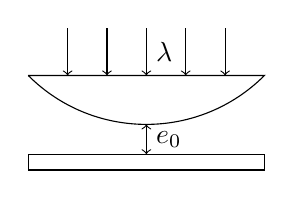
\begin{tikzpicture}
    \draw (-1.5,0) rectangle (1.5,.2);
    \draw (-1.5,1.2) arc (-135:-45:{1.5*sqrt(2)}) -- (-1.5,1.2);
    \draw [ <-> ] (0,{2.7 - 1.5*sqrt(2)}) -- node [ right ] {$e_0$} (0,.2);
    \foreach \i in {-2,-1,0,1,2}
      \draw [ ->, xshift = \i*.5cm ] (0,1.8) -- (0,1.2);
    \node [ right ] at (0,1.5) {$\lambda$};
  \end{tikzpicture}
\end{textfig}
\scratch[1ex]
\begin{solution}
  透镜下表面和平板玻璃表面之间的光程差
  $\delta = 2\ab(e_0 + R - \sqrt{R^2 - r_k^2}) - \lambda/2
  \approx 2(e_0 + r_k^2/2R) - \lambda/2$.
  由干涉暗纹条件
  $\delta = (2k - 1)\lambda/2$ 得第 $k$ 条暗纹半径 $r_k = \sqrt{R(k\lambda - 2e_0)}$.
\end{solution}

\begin{textfig}
  \begin{problem}
    如图所示，一平面简谐波沿 $x$ 轴正向传播. 已知 $P$ 点的振动方程为
    $y = A\cos(\omega t + \phi_0)$，则波的表达式为
    \begin{tasks}(2)
      \task[\true] $y = A\cos(\omega t - \omega x/u + \omega L/u + \phi_0)$
      \task $y = A\cos(\omega t - \omega x/u + \phi_0)$
      \task $y = A\cos(\omega t - \omega x/u - \omega L/u + \phi_0)$
      \task $y = A\cos(\omega t + \omega x/u - \omega L/u + \phi_0)$
    \end{tasks}
  \end{problem}
  \textfigsplit\centering
  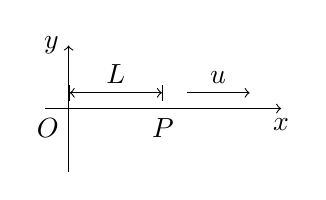
\begin{tikzpicture}
    \draw [ -> ] (-.3,0) -- (2.7,0) node [ below ] {$x$}
     node [ below ] at (1.2,0) {$P$};
    \draw [ -> ] (0,-.8) -- node [ below left ] {$O$} (0,.8)
     node [ left ] {$y$};
    \draw [ |<->| ] (0,.2) -- node [ above ] {$L$} (1.2,.2);
    \draw [ -> ] (1.5,.2) -- node [ above ] {$u$} ++ (.8,0);
  \end{tikzpicture}
\end{textfig}
\scratch[4ex]
\begin{solution}
  以 $P$ 为原点，波的表达式为 $y = A\cos(\omega t - \omega x/u + \phi_0)$，
  利用坐标变换 $x \to x - L$ 将坐标左移至 $O$ 点得波的表达式为
  $ y = A\cos(\omega t - \omega (x - L)/u + \phi_0)
      = A\cos(\omega t - \omega x/u + \omega L/u + \phi_0)
  $.
\end{solution}

\begin{problem}
  蝙蝠能利用超声波导航在洞穴里飞来飞去. 假如蝙蝠发出的超声波频率为 $\qty{39}\kHz$，
  当它以四十分之一声速（不用在意声速的具体数值）的速度朝着表面平直的岩壁飞去，
  则它听到的从岩壁反射回来的超声波频率为
  \begin{tasks}(4)
    \task $\qty{37}\kHz$
    \task $\qty{38}\kHz$
    \task $\qty{40}\kHz$
    \task[\true] $\qty{41}\kHz$
  \end{tasks}
\end{problem}
\scratch[8ex]
\begin{solution}
  整个过程分声波入射和反射两个阶段.
  由于两个阶段分别作为发射源 (Source) 的和观察者 (Observer) 的蝙蝠均接近，
  所以 $v_o = -v_s = u/40$. 根据多普勒效应公式得
  \[
    f = \frac{u \pm v_o}{u \mp v_s} f_0 = \frac{1 + 1/40}{1 - 1/40} f_0
      = \qty{41}\kHz
  \]
\end{solution}

\begin{textfig}
  \begin{problem}
    设沿弦线传播的入射波的表达式为 $y_1 = A\cos[2\pi(t/T - x/\lambda) + \phi]$，
    波在 $x = L$ 处（$B$点）发生反射，反射点位固定端（如图）.
    设波在传播和反射过程中振幅不变，则反射波的表达式为
    \begin{tasks}(2)
      \task $A\cos[2\pi(t/T - x/\lambda) + 4\pi L/\lambda + \phi - \pi]$
      \task $A\cos[2\pi(t/T + x/\lambda) + 2\pi L/\lambda + \phi - \pi]$
      \task[\true] $A\cos[2\pi(t/T + x/\lambda) - 4\pi L/\lambda + \phi + \pi]$
      \task $A\cos[2\pi(t/T + x/\lambda) + 4\pi L/\lambda + \phi + \pi]$
    \end{tasks}
  \end{problem}
  \textfigsplit\centering
  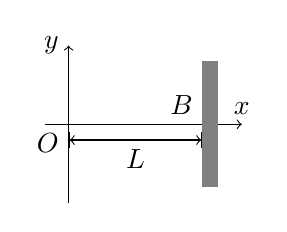
\begin{tikzpicture}
    \draw [ -> ] (-.3,0) -- (2.2,0) node [ above ] {$x$};
    \draw [ -> ] (0,-1) -- node [ below left ] {$O$} (0,1) node [ left ] {$y$};
    \fill [ gray ] (1.7,-.8) rectangle (1.9,.8);
    \draw [ |<->| ] (0,-.2) -- node [ below ] {$L$} (1.7,-.2)
     node [ above left ] at (1.7,0) {$B$};
  \end{tikzpicture}
\end{textfig}
\scratch[12ex]
\begin{solution}
  带入 $x = L$ 得入射波在 $B$ 点处的振动方程为
  $y (L,t) = A\cos(2\pi t/T - 2\pi L/\lambda + \phi)$.
  考虑反射半波损失，以 $B$ 点为原点，反射波的波函数为
  $y (x',t) = A\cos[2\pi(t/T + x'/\lambda) - 2\pi L/\lambda + \phi]$.
  做坐标变换 $x' \to x - L$，将原点平移至 $O$ 处得反射波的表达式为
  $ y (x,t) = A\cos[2\pi(t/T + x/\lambda) - 4\pi L/\lambda + \phi]$.
\end{solution}

\begin{problem}
  一平面简谐波在弹性媒质中传播，在媒质质元从最大位移处回到平衡位置的过程中
  \begin{tasks}(2)
    \task 它的势能转换成动能
    \task 它的动能转换成势能
    \task! 它把自己的能量传给相邻的一段媒质质元，其能量逐渐减小
    \task![\true] 它从相邻的一段媒质质元获得能量，其能量逐渐增加
  \end{tasks}
\end{problem}
\scratch[4ex]
\begin{solution}
  机械波中质元的动能、势能同时增加/减少，在最大位移处质元的动能、势能均最小，
  所以它从相邻的一段媒质质元获得能量，其能量逐渐增加.
\end{solution}

\begin{textfig}
  \begin{problem}
    用波长为 $\lambda$ 的单色光垂直照深如图所示的劈形膜（$n_1 > n_2 > n_3$），
    观察反射光干涉. 从劈形膜尖顶开始算起，第二条明纹中心所对应的膜厚度 $e =$
    \begin{tasks}(4)
      \task[\true] $\lambda/2n_2$
      \task $\lambda/n_2$
      \task $4\lambda/3n_2$
      \task $3\lambda/4n_2$
    \end{tasks}
  \end{problem}
  \textfigsplit\centering
  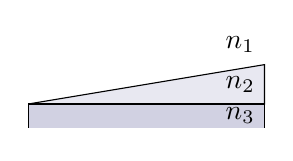
\begin{tikzpicture}
    \node [ left ] at (3,.75) {$n_1$};
    \filldraw [ fill = MidnightBlue!10 ] (0,0) -- (3,0) -- (3,.5) -- cycle
     node [ left ] at (3,.25) {$n_2$};
    \filldraw [ fill = MidnightBlue!20 ] (0,-.3) -- (0,0) -- (3,0) -- (3,-.3)
     node [ left ] at (3,-.15) {$n_3$};
  \end{tikzpicture}
\end{textfig}
\scratch[4ex]
\begin{solution}
  由于 $n_1 > n_2 > n_3$，所以上下表面均有半波损失，
  两表面的光程差为 $\delta = 2n_2e = k\lambda$.
  由于劈尖顶端光程差为 $0$，所以顶端为第一条明纹，则第二条明纹中心所对应的厚度为
  $e = (2 - 1)\lambda/2n_2 = \lambda/2n_2$.
\end{solution}

\begin{problem}
  关于光程，下列说法正确的是
  \begin{tasks}
    \task 假如光在真空中走过路程 $d$，则在相同时间内，光在介质中走过的路程 $d'$ 叫做光程.
    \task[\true] 假如光在介质中走过路程 $d$，则在相同时间内，
      光在真空中走过的路程 $d'$ 叫做光程.
    \task 光在真空中走过的路程乘以介质的折射率叫做光在介质里的光程.
    \task 在相同时间内，一束波长为 $\lambda$ 的单色光在空气中和在玻璃中，
    传播的路程不相等，走过的光程不相等.
  \end{tasks}
\end{problem}
\scratch[1ex]
\begin{solution}
  按照光程的定义，B选项正确. D选项中光在相同时间内，不同介质中，走过的光程相等.
\end{solution}

\begin{textfig}
  \begin{problem}
    声音在暖空气中比在冷空气中传播得快（即波长更长）. 想象一个由北向南分布的锋面，
    暖空气在锋面的西边，冷空气在锋面的东边. 一列在暖空气中向东北方向传递的声波遇到了这一锋面，
    则当此声波进入冷空气时，将如何改变方向？（提示：可利用惠更斯原理判断声波的波面将如何偏转）
    \begin{tasks}(2)
      \task[\true] 声波的方向将向东偏转
      \task 声波的方向将向北偏转
      \task 声波的方向不会偏转
      \task 声波将沿原路返回
    \end{tasks}
  \end{problem}
  \textfigsplit\centering
  \begin{tikzpicture}
    \draw [ dashed ] (-1,0) node [ left ] {西} -- (1,0) node [ right ] {东};
    \draw (0,-1) -- (0,1) node [ above ] {锋面};
  \end{tikzpicture}
\end{textfig}
\scratch
\begin{solution}
  将声波在锋面附近的传播与光在不同介质中的传播类比.
  由于声音在暖空气中比在冷空气中传播得快，所以暖空气为光疏介质，冷空气为光密介质.
  根据光的折射定律可知声波的方向将向东偏转.
\end{solution}
  
\section{填空题（每空2分，共18分）}

\begin{problem}
  一弹簧振子做简谐振动，其动能的变化频率为 $f$. 则其振动频率为 \result{$f/2$}.
\end{problem}
\scratch
\begin{solution}
  动能和势能变化趋势相反，所以二者变化频率相同. 势能 $E_p\propto x^2$，由于 $E$ 是周期为$T = 1/f$ 的余弦函数，所以 $x$ 的周期为 $2T$，频率为 $1/2T = f/2$.
\end{solution}

\begin{textfig}
  \begin{problem}
    图示一平面简谐机械波在 $t$ 时刻的波形曲线. 若此时 $A$ 点处某媒质质元的振动动能在增大，
    则波沿 $x$ 轴 \result{负方向} （正方向/负方向）传播.
  \end{problem}
  \scratch
\begin{solution}
    由于 $A$ 点处媒质质元的振动动能在增大，所以 $A$ 点正在往靠近平衡点方向运动，
    所以波沿 $x$ 轴 负方向传播.
\end{solution}
  \textfigsplit\centering
  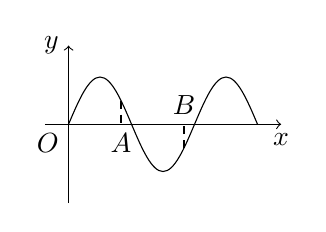
\begin{tikzpicture}
    \draw [ -> ] (-.3,0) -- (2.7,0) node [ below ] {$x$};
    \draw [ -> ] (0,-1) -- node [ below left ] {$O$} (0,1)
     node [ left ] {$y$};
    \draw (0,0) sin (.4,.6) cos (.8,0) sin (1.2,-.6)
                cos (1.6,0) sin (2,.6) cos (2.4,0);
    \draw [ densely dashed ] (2/3,.3) -- (2/3,0) node [ below ] {$A$};
    \draw [ densely dashed, xshift = .8cm ] (2/3,-.3) -- (2/3,0)
     node [ above ] {$B$};
  \end{tikzpicture}
\end{textfig}

\begin{problem}
  某科研院所进行海底探测时，利用声纳装置向海水中发出超声波 
  $y = \num{1.2e-3} \cos(\num{3.14e5} t + 220x)~\text{(SI)}$，
  则此波的频率 $f = $ \result{$\qty{5e4}\Hz$}，
  波长 $\lambda = $ \result{$\qty{0.0285}\m$}，
  海水中声速 $u = $ \result{$\qty{1428}{\m/\s}$}.
\end{problem}
\scratch
\begin{solution}
  将波函数改写为
  $ y = A\cos\ab[\omega\ab(t + \frac xu) + \phi]
      = 0.02\cos\ab[\num{3.14e5} \times \ab(t + \frac{x}{1428})]
  $，由此得海水中声速 $u = \qty{1428}{\m/\s}$，频率 $f = \qty{5e4}{\Hz}$，
  波长 $\lambda = 2\pi u/\omega = \qty{0.0285}\m$.
\end{solution}

\begin{problem}
  点光源的薄膜等倾干涉条纹是内疏外密的同心圆环，
  凸透镜及平玻璃板构成的牛顿环装置在平行光垂直照射时，条纹也是内疏外密的同心圆环.
  等倾干涉条纹级次由内向外 \result{变低} （变高/变低）；
  牛顿环干涉条纹级次由内向外 \result{变高} （变高/变低）.
\end{problem}
\scratch
\begin{solution}
  等倾干涉明纹所满足的关系为
  $\delta = 2e\sqrt{n^2 - n_1^2\sin^2i} + (\lambda/2) = k\lambda$，
  由此可知 $k$ 与入射角 $i$ 成负相关，所以等倾干涉条纹级次由内向外变低.
  牛顿环干涉明纹半径 $r_k = \sqrt{R(k\lambda + \lambda/2 - 2h)}$，
  由此可知 $k$ 与半径成正相关，所以牛顿环干涉条纹级次由内向外变高.
\end{solution}

\begin{problem}
  一双缝干涉装置，在空气中观察时干涉条纹间距为 $\qty{1.0}\mm$. 若整个装置放在水中，
  干涉条纹的间距将为 \result{$\qty{0.75}\mm$}（设水的折射率为 $4/3$）.
\end{problem}
\scratch
\begin{solution}
  装置放在水中会讲光的波长由 $\lambda$ 减小到 $\lambda/n = 0.75\lambda$，
  由于双缝干涉条纹间距 $\Delta x \propto \lambda$，
  所以放在水中后条纹间距 $\Delta x' = \Delta x/n = \qty{0.75}\mm$.
\end{solution}

\begin{problem}
  在单缝夫琅和费衍射实验中，波长为 $\lambda$ 的单色光垂直入射在宽度 $a = 6\lambda$
  的单缝上，对应于衍射角为 $\qty{30}\degree$ 的方向，
  单缝波阵面可分成半波带数目为 \result{$6$}.
\end{problem}
\scratch
\begin{solution}
  由于衍射条纹公式 $a\sin\theta = k\lambda$ 得 $k = 3$，所以半波带数目 $2k = 6$.
\end{solution}

\section{解答题（共46分）}

\begin{problem}[本题12分]
  一物体作简谐振动，其速度最大值 $v_m = \qty{3e-2}{\m/\s}$，其振幅 $A = \qty{2e-2}\m$.
  若 $t = 0$ 时，物体位于平衡位置且向 $x$ 轴的负方向运动. 求
  \begin{tasks}[ label = \arabic*. ](3)
    \task 振动周期 $T$.
    \task 加速度的最大值 $a_m$.
    \task 振动方程的表达式.
  \end{tasks}
\end{problem}
\scratch[10ex]
\begin{solution}\leavevmode
  \begin{enumerate}
    \item 振动角频率 $\omega = v/A = \qty{1.5}{\radian/\s}$，
    所以振动周期 $T = 2\pi/\omega = \qty{4.19}\s$.
    \item 加速度的最大值 $a_m = \omega^2A =\qty{4.5e-2}{\m/\s^2}$.
    \item $t = 0$ 时，$x = 0$，$v < 0$，所以物体的初相为 $\pi/2$.
    振动方程的表达式为 $y = \num{2e-2}\cos(1.5 t + \pi/2)$.
  \end{enumerate}
\end{solution}

\begin{problem}[本题12分]
  在均匀介质中，一列余弦波沿 $Ox$ 轴传播，波动方程为 $y = A\cos(2\pi t + \pi x/3)$，
  在 $x = \qty1\m$ 处发生反射，反射点为固定端，则求反射波和入射波产生的驻波表达式，
  及驻波的波腹点坐标.
\end{problem}
\scratch[20ex]
\begin{solution}\leavevmode
  \begin{itemize}
    \item 波速 $u = \qty6{\m/\s}$，固定端的振动方程为
    $y_1(1,t) = A\cos(2\pi t + \pi/3)$.
    \item 考虑反射半波损失，以固定端为原点，加入传播项得反射波波函数
    $y_2(x',t) = A\cos[2\pi(t - x'/6) + 4\pi/3]$.
    \item 做坐标变换 $x' \to x - 1$ 得以 $x = 0$ 为原点的反射波波函数
    $y_2(x,t) = A\cos[2\pi t - \pi x/3 + 5\pi/3]$.
    \item 驻波表达式
    $y = y_1 + y_2 = 2A\cos(2\pi t + 5\pi/6)\cos(\pi x/3 - 5\pi/6)$.
    \item 波腹坐标：$\pi x/3 - 5\pi/6 = k\pi$，
    $x = 3k + 5/2,~ k = 1,~ 2,~ 3,~ \ldots$.
  \end{itemize}
\end{solution}

\begin{textfig}
  \begin{problem}[本题6分]
    如图所示，将一转动惯量为 $I$ 的电偶极矩 $\bm p = q\bm l$ 放置在均匀电场 $\bm E$中，
    让它在平衡位置（稳定平衡点）附近转过微小角度并释放，证明其做近似
    $\theta = \theta_0 \cos(\omega t + \phi)$ 的简谐振动，并给出其振动频率.
    （提示：在小角度下 $\theta \approx \sin\theta$，转动定律 $M = I\beta$）.
  \end{problem}
  \textfigsplit\centering
  \begin{tikzpicture}
    \foreach \i in {-7,-5,...,7}
      \draw [ ->, yshift = \i*.15cm, gray!80 ] (-1.6,0) -- (1.6,0);
    \node
      [ shade, ball color = MidnightBlue!20,
        circle, minimum width = .15cm, scale = .6
      ] (a) at ({-cos(37)},{-sin(37)}) {$\scriptstyle -$};
    \node
      [ shade, ball color = DarkGreen!20,
        circle, minimum width = .15cm, scale = .6
      ] (b) at ({cos(37)},{sin(37)}) {$\scriptstyle +$};
    \draw [ -> ] (a) --
     node [ fill, circle, minimum width = 1.6pt, inner sep = 0pt ] {}
     node [ above ] {$O$} (b) node [ above left ] {$\bm p$};
    \draw [ -> ] (a) --++ (-.8,0) node [ above right ] {$\bm F_-$};
    \draw [ -> ] (b) --++ (.8,0) node [ below left ] {$\bm F_+$};
    \draw [ dashed, gray ] (a) --++ (1,0) coordinate (c);
    \pic [ "$\theta$", draw, angle eccentricity = 2, angle radius = .25cm ]
     { angle=c--a--b };
  \end{tikzpicture}
\end{textfig}
\scratch[12ex]
\begin{solution}
  \begin{proof}
    以 $O$ 点为支点，电偶极子所受外力矩为
    $|\bm M| = |-\bm p \times \bm E| = -qlE\sin\theta \approx -qlE\theta$，
    负号表示力矩方向垂直于纸面向内. 由于电偶极子所受回复力矩正比于广义坐标 $\theta$，
    所以其做近似 $\theta = \theta_0 \cos(\omega t + \phi)$ 的简谐振动.
  \end{proof}
  由转动定律 $M = I\ddot\theta$ 得
  \[
    -qlE\sin\theta \approx -qlE\theta = I\ddot\theta,~
    \ddot\theta + \frac{qlE}{I}\theta = 0
  \]
  所以其振动频率为 $\omega = \sqrt{qlE/I}$.
\end{solution}

\begin{problem}[本题8分]
  一个非常薄的肥皂膜（$n = 1.33$），其厚度远远小于可见光波长，那么它看起来将是黑色的，
  它看起来根本不反射光，为什么？与之相比，一层同样厚度的、附着在玻璃（$n = 1.50$）上的肥皂水（$n = 1.33$）看起来将会相当有光泽，为什么会有这样的区别？
\end{problem}
\scratch[8ex]
\begin{solution}\leavevmode
  \begin{itemize}
    \item 在空气中时，只有从其前表面反射的光存在半波损失，从其前、后表面反射的光的光程差为
    $2ne + \lambda/2 \to \lambda/2$，满足干涉相消条件，所以看起来根本不反射光.
    \item 附着在玻璃上时，从其前、后表面反射的光均存在半波损失，光程差为 $\delta = 2ne \to 0$，满足干涉相长条件，所以看起来非常有光泽.
  \end{itemize}
\end{solution}

\begin{problem}[本题8分]
  广播因其波长较短，因而人类在很长一段时间内都没有发现其衍射现象.
  而声波波长较长，可以非常容易的进行声波的衍射实验. 假设一频率为$\qty{1250}\Hz$
  的声音通过 $\qty{0.8}\m$ 宽的门离开隔音房间向外传播.
  屋外的人站在相对于门道中垂线的某些角度上，收到的声音就几乎趋向于 $0$（即单缝衍射暗纹），
  假设空气中声速取 $\qty{340}{\m/\s}$，假设声源与人都距离门道足够远，因此夫琅和费衍射适用，
  忽略反射效应，则这些听不到声音的角度，最小的角度为多少？
\end{problem}
\scratch[6ex]
\begin{solution}
  由单缝衍射暗纹所满足的公式 $a\sin\theta = k\lambda = ku/f$ 得听不到声音的衍射角为 
  $\theta = \sin^{-1}(ku/fa)$，取 $k = 1$ 得其极小值
  $\theta_{\min} = \arcsin(u/fa) = \sin^{-1} 0.34$.
\end{solution}